\chapter{Service-Based Architecture}
\label{bab:layanan}

\section*{Tujuan Pembelajaran}

\begin{enumerate}
  \item Menjelaskan tiga ciri service-based architecture, yaitu layanan
    berbutir kasar, basis data yang dipakai bersama, dan gerbang antarmuka di
    depannya.
  \item Membedakan pembagian berbutir kasar tersebut dari monolit berlapis
    maupun dari mikroservis, lalu menentukan kapan masing-masing layak
    dipilih.
  \item Mengukur tambahan waktu tanggap akibat lompatan jaringan, jumlah
    permintaan yang selamat ketika satu layanan mati, dan biaya mengubah skema
    basis data bersama.
\end{enumerate}

\section{Pendahuluan}

Pemecahan sebuah aplikasi menjadi beberapa unit yang dijalankan terpisah
sering diperbincangkan sebagai pilihan antara dua ujung. Ujung pertama adalah
monolit, yaitu seluruh kemampuan berada di dalam satu unit. Ujung kedua adalah
mikroservis, yaitu setiap kemampuan kecil berdiri sebagai layanan tersendiri
beserta basis datanya sendiri. Ruang di antara kedua ujung itu jarang dibahas,
padahal justru di situlah banyak sistem nyata berada.

Service-based architecture menempati ruang antara tersebut. Aplikasinya
dipecah menjadi sedikit layanan domain yang berbutir kasar, lazimnya empat
sampai duabelas. Setiap layanan berjalan sebagai proses tersendiri dan
dipanggil lewat Hypertext Transfer Protocol (HTTP). Basis datanya tetap satu
dan dipakai bersama seluruh layanan, dan ciri terakhir itulah yang
membedakannya dari mikroservis.

Pembagian tersebut menarik sebab harganya dapat diukur dari tiga arah
sekaligus, yaitu waktu tanggap, ketahanan terhadap kegagalan, dan biaya
perubahan. Pembahasan bab ini mengikuti kerangka yang disusun Richards dan
Ford~\cite{richards2020fundamentals}, serta saran Fowler agar sebuah sistem
dimulai sebagai monolit lebih dahulu sebelum
dipecah~\cite{fowler2015monolithfirst}.

\section{Butir Layanan yang Kasar}

Butir sebuah layanan menyatakan seberapa banyak kemampuan yang dibungkusnya.
\textbf{Butir kasar} berarti satu layanan memegang satu bidang domain utuh,
misalnya seluruh urusan penagihan. \textbf{Butir halus} berarti satu layanan
hanya memegang satu tindakan, misalnya menghitung pajak sebuah tagihan.
Service-based architecture memilih butir kasar, sehingga jumlah layanannya
tetap sedikit.

Gambar~\ref{fig:butir-layanan} menempatkan ketiga bentuk pada satu garis yang
sama. Yang berubah dari kiri ke kanan ada dua, yaitu jumlah unit yang
dijalankan dan letak basis datanya.

\begin{figure}[htbp]
  \centering
  \begin{tikzpicture}[
    kotak/.style={draw, rounded corners=2pt, minimum width=3.4cm,
      minimum height=1.0cm, align=center, font=\scriptsize\bfseries},
    data/.style={draw, rounded corners=2pt, minimum width=3.4cm,
      minimum height=0.6cm, align=center, font=\tiny},
    panah/.style={-{Stealth[length=2mm]}, thick}
  ]
    \node[kotak, fill=blue!8] (mono) {Monolit berlapis\\
      {\tiny\mdseries satu unit dijalankan}};
    \node[kotak, fill=praditagreen!25, right=0.45cm of mono] (layanan)
      {Service-based\\
      {\tiny\mdseries 4 sampai 12 layanan domain}};
    \node[kotak, fill=green!10, right=0.45cm of layanan] (mikro)
      {Mikroservis\\
      {\tiny\mdseries puluhan layanan kecil}};

    \node[data, fill=gray!18, below=0.55cm of mono] (dmono)
      {satu basis data};
    \node[data, fill=gray!18, below=0.55cm of layanan] (dlayanan)
      {satu basis data bersama};
    \node[data, fill=gray!18, below=0.55cm of mikro] (dmikro)
      {basis data per layanan};

    \draw[panah] (mono) -- (dmono);
    \draw[panah] (layanan) -- (dlayanan);
    \draw[panah] (mikro) -- (dmikro);
    \draw[panah] ([yshift=-0.35cm]dmono.south west)
      -- node[below, font=\tiny] {butir makin halus, jumlah unit makin banyak}
      ([yshift=-0.35cm]dmikro.south east);
  \end{tikzpicture}
  \caption{Tiga bentuk pembagian pada satu garis yang sama. Service-based
    architecture memecah prosesnya, tetapi belum memecah basis datanya}
  \label{fig:butir-layanan}
\end{figure}

Analogi yang mendekati adalah kantor layanan mahasiswa. Ruangannya punya tiga
loket, yaitu loket keuangan, loket akademik, dan loket kemahasiswaan. Ketiga
loket melayani antrean sendiri-sendiri, sehingga loket yang tutup tidak
menghentikan loket sebelahnya. Akan tetapi berkas mahasiswa tetap disimpan di
satu lemari arsip di belakang ruangan, dan ketiga petugas mengambil dari lemari
yang sama. Lemari itulah basis data bersama pada bab ini.

Pembagian tersebut menentukan letak setiap keputusan.
Tabel~\ref{tab:butir-layanan} merangkum perbedaan ketiga bentuk pada empat hal
yang paling sering ditanyakan.

\begin{table}[htbp]
  \centering
  \caption{Perbedaan monolit berlapis, service-based, dan mikroservis}
  \label{tab:butir-layanan}
  \begin{tabularx}{\textwidth}{|l|X|X|X|}
    \hline
    \textbf{Yang dibandingkan} & \textbf{Monolit berlapis} & \textbf{Service-based} & \textbf{Mikroservis} \\
    \hline
    Unit yang dijalankan & Satu & Empat sampai duabelas & Puluhan \\
    \hline
    Basis data & Satu & Satu, dipakai bersama & Terpisah per layanan \\
    \hline
    Pemanggilan antar bidang & Pemanggilan fungsi & Lewat jaringan & Lewat jaringan \\
    \hline
    Yang menjadi mahal & Menjalankan ulang seluruhnya & Mengubah skema bersama & Menjaga data tetap padu \\
    \hline
  \end{tabularx}
\end{table}

Baris terakhir tabel tersebut yang paling menentukan. Mikroservis memutus
hubungan lewat basis data, sehingga setiap layanan bebas mengubah skemanya
sendiri. Kebebasan itu dibayar dengan pekerjaan menjaga data tetap padu antar
layanan, dan Bab~13 membahasnya tersendiri. Service-based architecture menolak
membayar harga tersebut, lalu membayar harga yang lain.

\section{Gerbang, Layanan Domain, dan Basis Data Bersama}

Susunannya terdiri atas tiga bagian. \textbf{Gerbang} menerima permintaan
klien lalu meneruskannya, dan tidak memuat satu pun aturan bisnis.
\textbf{Layanan domain} memuat aturan satu bidang, dan pada contoh bab ini
jumlahnya tiga, yaitu kurs, pemesanan, dan penagihan. \textbf{Basis data
bersama} menyimpan seluruh tabel, dan ketiga layanan membukanya sebagai berkas
yang sama.

Contoh bab ini menjalankan ketiga layanan pada nomor porta yang berbeda, yaitu
8101, 8102, dan 8103, sedangkan gerbangnya di porta 8100. Versi monolit
menempati satu porta saja, yaitu 8000, dan memanggil ketiga bidang sebagai
fungsi biasa. Kode bidangnya sama persis pada kedua versi, sehingga yang
dibandingkan benar-benar letak prosesnya.

Gambar~\ref{fig:kelas-layanan} memperlihatkan hubungan ketiganya. Perhatikan
dua panah yang berangkat dari layanan penagihan, sebab layanan itu menulis
tabel tagihan sekaligus membaca tabel pesanan.

\begin{figure}[htbp]
  \centering
  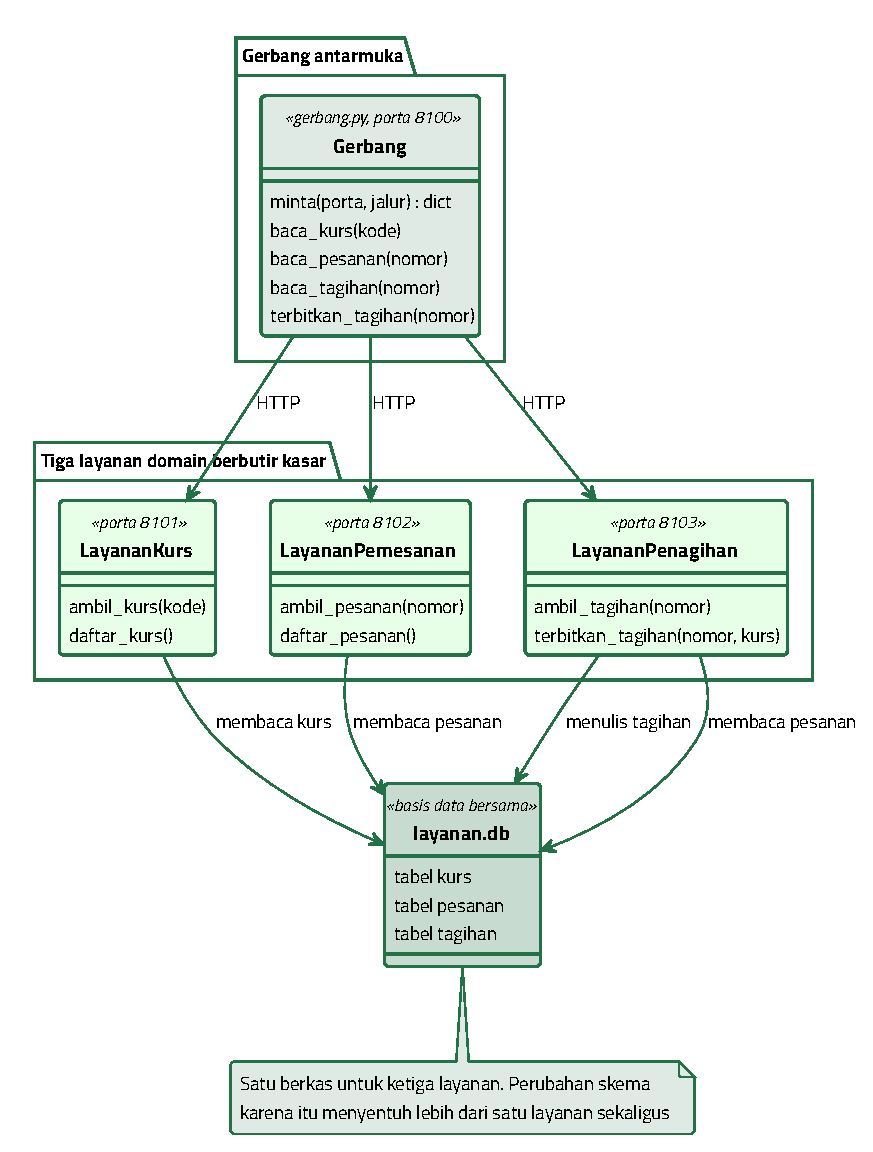
\includegraphics[width=0.9\textwidth, height=0.62\textheight,
    keepaspectratio]{kelas-layanan.pdf}
  \caption{Gerbang mengenal ketiga layanan lewat nomor porta, bukan lewat
    impor. Ketiga layanan menunjuk berkas basis data yang sama}
  \label{fig:kelas-layanan}
\end{figure}

Versi monolit memanggil ketiga bidang sebagai fungsi biasa, dan
Listing~\ref{lst:monolit} memperlihatkan seluruh jalur gabungannya. Panjangnya
tiga baris, sebab tidak ada permintaan yang perlu disusun maupun jawaban yang
perlu diuraikan.

\begin{lstlisting}[style=PythonStyle, caption={Jalur gabungan pada versi
  monolit, tersedia di \berkas{sources/chapter11/monolit.py}},
  label=lst:monolit]
@aplikasi.post("/pesanan/<int:nomor>/tagihan")
def terbitkan_tagihan(nomor: int) -> dict:
  """Melayani permintaan gabungan yang menyentuh ketiga bidang sekaligus."""
  pesanan = domain_pemesanan.ambil_pesanan(nomor)
  kurs = domain_kurs.ambil_kurs(pesanan["mata_uang"])
  tagihan = domain_penagihan.terbitkan_tagihan(nomor, kurs["nilai"])
  return {
    "pesanan": pesanan,
    "kurs": kurs,
    "tagihan": tagihan,
    "lompatan": alamat.LOMPATAN_KLIEN,
  }
\end{lstlisting}

Bagian yang paling layak diperhatikan justru ada di bidang penagihan.
Listing~\ref{lst:penagihan} memperlihatkan bahwa bidang tersebut membaca tabel
pesanan langsung dari basis data bersama, bukan bertanya kepada bidang
pemesanan.

\begin{lstlisting}[style=PythonStyle, caption={Pembacaan silang lewat basis
  data bersama, tersedia di
  \berkas{sources/chapter11/domain_penagihan.py}}, label=lst:penagihan]
AMBIL_PESANAN_UNTUK_TAGIHAN = """
SELECT nomor, nominal, status
FROM pesanan
WHERE nomor = ?
"""


def terbitkan_tagihan(nomor_pesanan: int, nilai_kurs: float) -> dict:
  """Menghitung lalu menyimpan tagihan satu pesanan dalam rupiah."""
  koneksi = basis_data.buka_koneksi()
  try:
    baris = koneksi.execute(
      AMBIL_PESANAN_UNTUK_TAGIHAN, (nomor_pesanan,)).fetchone()
    if baris is None:
      raise kesalahan.TidakDitemukan(f"pesanan {nomor_pesanan} tidak terdaftar")
    if baris["status"] == basis_data.STATUS_BATAL:
      raise kesalahan.AturanDilanggar(
        f"pesanan {nomor_pesanan} sudah dibatalkan, tidak dapat ditagih")
\end{lstlisting}

Pembacaan silang tersebut murah dan menggoda. Satu kueri sudah cukup, tanpa
lompatan jaringan dan tanpa kesepakatan antarmuka. Mikroservis melarangnya,
sebab tabel pesanan hanya boleh disentuh pemiliknya. Service-based architecture
mengizinkannya, dan izin itu punya dua akibat. Pertama, aturan bisnis tetap
dapat dijalankan utuh walaupun prosesnya sudah dipecah. Kedua, nama kolom pada
tabel pesanan kini dipakai dua bidang sekaligus.

Akibat kedua itulah yang menimbulkan persoalan berikutnya. Pertanyaannya,
berapa harga yang dibayar sebuah permintaan ketika ketiga bidang tersebut
dipisahkan menjadi tiga proses.

\section{Harga Satu Lompatan Jaringan}

Setiap pemanggilan lewat jaringan menambah pekerjaan yang tidak ada pada
pemanggilan fungsi, yaitu penyusunan permintaan, pengiriman, penguraian
jawaban, dan penantian. Fielding menempatkan biaya komunikasi itu sebagai
pembatas utama arsitektur berbasis jaringan, sebab sifat jaringan tidak dapat
disembunyikan dari perancangnya~\cite{fielding2000architectural}.

Contoh bab ini memakai satu permintaan yang menyentuh ketiga bidang sekaligus,
yaitu menerbitkan tagihan untuk pesanan nomor satu. Versi monolit
menyelesaikannya dengan tiga pemanggilan fungsi di dalam satu proses. Versi
service-based menempuh tiga lompatan jaringan tambahan untuk pekerjaan yang
sama persis. Gambar~\ref{fig:sekuens-layanan} membandingkan keduanya.

\begin{figure}[htbp]
  \centering
  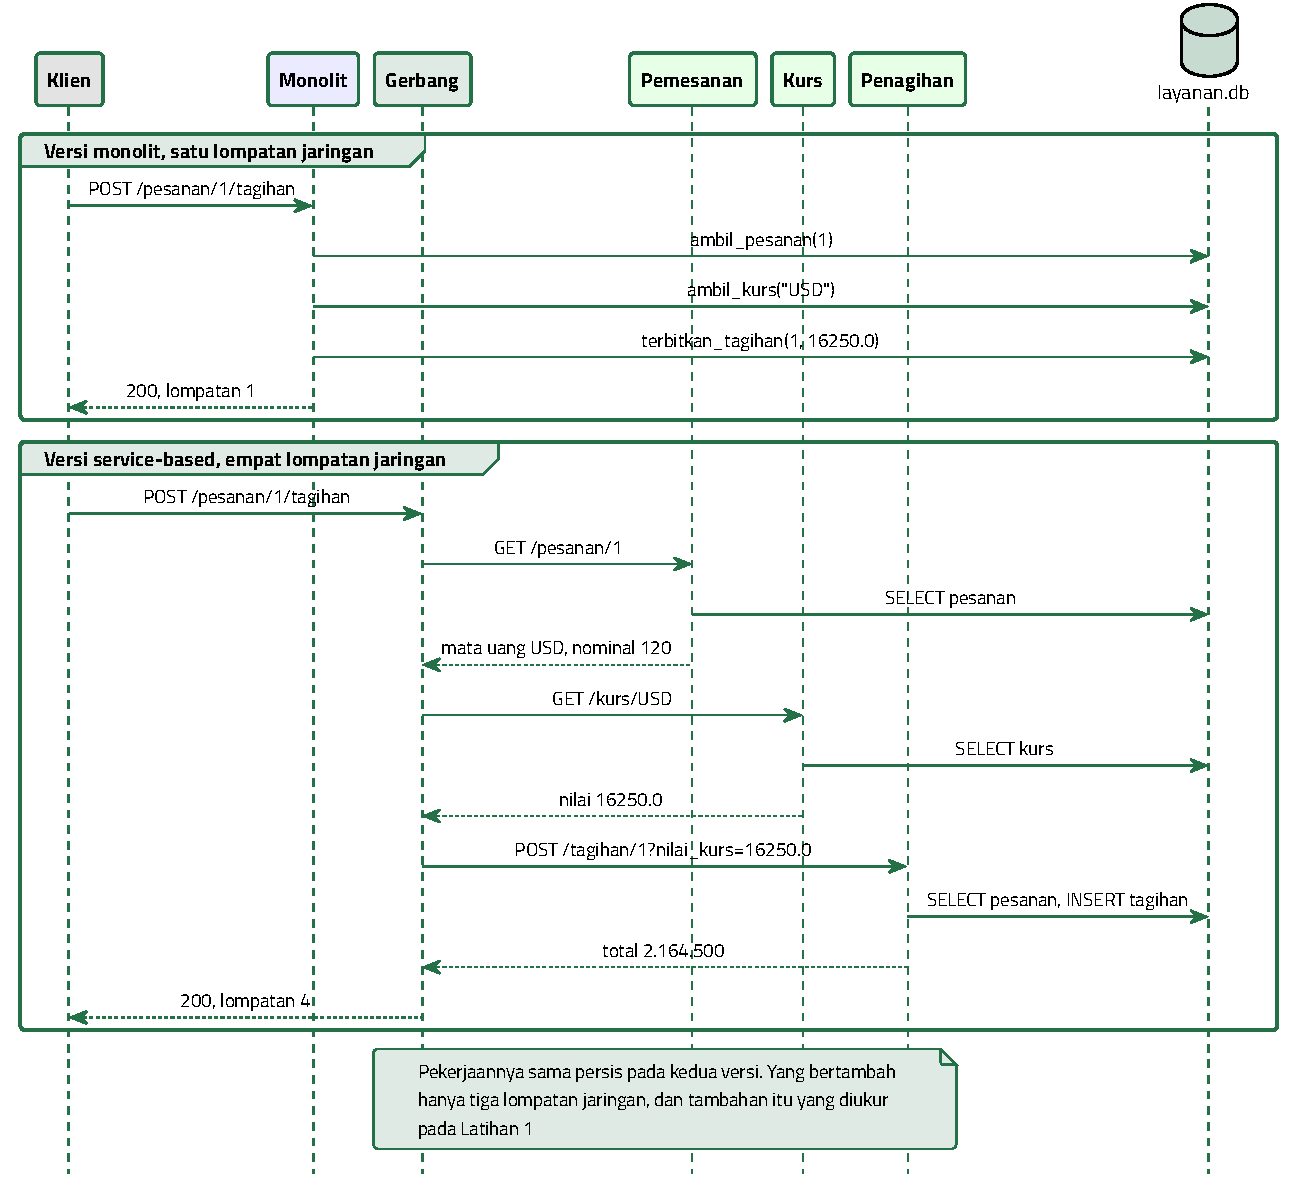
\includegraphics[width=\textwidth, height=0.62\textheight,
    keepaspectratio]{sekuens-layanan.pdf}
  \caption{Permintaan yang sama pada kedua versi. Yang bertambah hanya tiga
    lompatan jaringan, sedangkan pekerjaannya tidak berubah}
  \label{fig:sekuens-layanan}
\end{figure}

Jalur gabungan pada gerbang memuat pekerjaan tambahan itu secara terang-terangan.
Listing~\ref{lst:gerbang} memperlihatkan ketiga panggilan keluarnya, dan
ketiganya berjalan berurutan sebab nilai kurs baru diketahui sesudah pesanannya
terbaca.

\begin{lstlisting}[style=PythonStyle, caption={Jalur gabungan pada gerbang,
  tersedia di \berkas{sources/chapter11/gerbang.py}}, label=lst:gerbang]
@aplikasi.post("/pesanan/<int:nomor>/tagihan")
def terbitkan_tagihan(nomor: int) -> dict:
  """Merangkai jawaban gabungan dari ketiga layanan domain sekaligus."""
  pesanan = minta(alamat.PORTA_PEMESANAN, f"/pesanan/{nomor}")
  kurs = minta(alamat.PORTA_KURS, f"/kurs/{pesanan['mata_uang']}")
  tagihan = minta(alamat.PORTA_PENAGIHAN, f"/tagihan/{nomor}", "POST",
                  {"nilai_kurs": kurs["nilai"]})
  return {
    "pesanan": pesanan,
    "kurs": kurs,
    "tagihan": tagihan,
    "lompatan": (alamat.LOMPATAN_KLIEN + pesanan["lompatan"]
                 + kurs["lompatan"] + tagihan["lompatan"]),
  }
\end{lstlisting}

Angka lompatan pada baris terakhir tidak ditulis sebagai tetapan, melainkan
dijumlahkan dari jawaban setiap layanan. Cara itu dipilih agar jumlahnya
terukur, bukan diyakini. Hasil pengukuran seratus lima puluh putaran tercantum
pada Tabel~\ref{tab:latensi}. Median versi service-based 1,8 kali median versi
monolit, dan angka lompatannya berbanding satu melawan empat.

\begin{table}[htbp]
  \centering
  \caption{Waktu tanggap satu permintaan gabungan, seratus lima puluh putaran}
  \label{tab:latensi}
  \begin{tabularx}{\textwidth}{|X|l|l|}
    \hline
    \textbf{Yang diukur} & \textbf{Monolit} & \textbf{Service-based} \\
    \hline
    Median & 5,03 ms & 9,07 ms \\
    \hline
    Persentil ke-95 & 5,87 ms & 10,89 ms \\
    \hline
    Terbesar & 9,74 ms & 29,68 ms \\
    \hline
    Lompatan jaringan per permintaan & 1 & 4 \\
    \hline
    Putaran lebih cepat & 150 dari 150 & 0 dari 150 \\
    \hline
  \end{tabularx}
\end{table}

Angka terbesar pada tabel tersebut perlu dibaca dengan hati-hati. Selisih
mediannya hanya 4,04 ms, sedangkan \textit{range} di dalam jalur monolit
sendiri mencapai 5,20 ms, yaitu 1,29 kali selisihnya. Menurut ukuran Bab~2,
perbandingan seperti itu biasanya menjadi alasan untuk menahan kesimpulan.

Dua angka lain justru menolak keraguan tersebut. Persentil ke-95 kedua jalur
tidak bertumpang tindih sama sekali, yaitu 5,87 ms melawan 10,89 ms.
Pencacahan per putaran bahkan mencatat 150 dari 150 putaran dimenangkan versi
monolit. Yang menggelembungkan \textit{range} ternyata satu putaran lambat,
sebab nilai terbesarnya 9,74 ms sedangkan persentil ke-95 hanya 5,87 ms. Satu
pencilan memang cukup untuk merusak \textit{range}, sehingga ukuran itu tidak
boleh dibaca sendirian.

Nilai terbesar pada jalur service-based memperlihatkan gejala yang lain lagi,
yaitu 29,68 ms atau hampir tiga kali persentil ke-95 jalurnya sendiri. Gejala
antrean seperti itu hanya muncul pada ekor sebaran. Empat proses yang saling
menunggu di satu laptop sesekali berebut giliran, dan kejadian yang jarang itu
tidak pernah terlihat pada rata-rata maupun median.

\section{Ketika Satu Layanan Mati}

Pemecahan proses menjanjikan sesuatu yang tidak dimiliki monolit, yaitu
kegagalan yang tertahan di satu tempat. Janji tersebut dapat diuji dengan cara
sederhana, yaitu mematikan satu bagian lalu mencacah permintaan yang masih
terlayani. Contoh bab ini memakai empat jenis permintaan, dan tiga di antaranya
menyentuh satu bidang saja.

Tabel~\ref{tab:kegagalan} memuat hasil ketiga keadaan yang diuji. Keadaan
pertama adalah keadaan sehat, sebagai pembanding.

\begin{table}[htbp]
  \centering
  \caption{Permintaan yang masih terlayani pada tiga keadaan}
  \label{tab:kegagalan}
  \begin{tabularx}{\textwidth}{|X|l|l|}
    \hline
    \textbf{Keadaan} & \textbf{Monolit} & \textbf{Service-based} \\
    \hline
    Seluruh proses hidup & 4 dari 4 & 4 dari 4 \\
    \hline
    Bidang kurs dimatikan & 0 dari 4 & 2 dari 4 \\
    \hline
    Basis data bersama dikunci & 0 dari 4 & 0 dari 4 \\
    \hline
  \end{tabularx}
\end{table}

Baris kedua memperlihatkan janji yang ditepati. Pada versi service-based,
bidang kurs berupa proses tersendiri, sehingga mematikannya menyisakan
permintaan baca pesanan dan baca tagihan. Pada versi monolit, bidang kurs tidak
punya proses sendiri, sehingga mematikannya berarti mematikan seluruh
aplikasi. Perlu dicatat bahwa permintaan terbitkan tagihan ikut gagal pada
kedua versi, sebab permintaan itu memang membutuhkan nilai kurs.

Baris ketiga memperlihatkan batas janji tersebut. Berkas basis data ditahan
dengan kunci penuh SQLite, lalu keempat permintaan dicoba lagi. Hasilnya nol
dari empat pada kedua versi. Memecah proses ternyata tidak dengan sendirinya
memecah titik kegagalan, sebab titik itu pindah ke berkas yang dipakai
bersama. Kembali ke analogi kantor tadi, menutup satu loket hanya memotong satu
antrean, sedangkan mengunci lemari arsip menghentikan ketiga loket sekaligus.

\section{Harga Basis Data Bersama}

Harga yang sebenarnya dari basis data bersama tidak muncul pada waktu tanggap,
melainkan pada biaya perubahan. Dua jenis perubahan perlu dibedakan.
\textbf{Perubahan di dalam satu bidang} tidak menyentuh bidang lain, misalnya
menambah ringkasan kurs. \textbf{Perubahan skema bersama} menyentuh setiap
bidang yang membaca tabelnya, misalnya mengganti nama sebuah kolom.

Kasus berikut memperlihatkan akibatnya. Sebuah tim memecah sistem pembayaran
kampus menjadi empat layanan yang memakai satu basis data. Pada suatu malam,
kolom \texttt{nominal} pada tabel pesanan diganti namanya menjadi
\texttt{nominal\_asing}, dan perubahan itu dijalankan bersama pembaruan layanan
pemesanan. Layanan pemesanan langsung berjalan normal. Layanan penagihan tidak,
sebab layanan itu masih memuat kueri lama yang menyebut kolom lama. Kegagalan
baru ketahuan keesokan paginya, yaitu ketika tagihan pertama hari itu
diterbitkan. Akibatnya, pembaruan satu layanan terpaksa ditarik kembali,
padahal kodenya sendiri tidak bersalah.

Biaya kedua jenis perubahan tersebut dihitung skrip
\texttt{biaya\_perubahan.py} tanpa menyunting berkas sumber sama sekali.
Perubahannya diterapkan pada salinan di dalam memori, diperiksa dengan
\texttt{compile}, lalu dibandingkan memakai \texttt{difflib}. Jumlah proses yang
harus dijalankan ulang dihitung dari pernyataan \texttt{import} setiap proses,
bukan dikira-kira. Tabel~\ref{tab:biaya} memuat hasilnya.

\begin{table}[htbp]
  \centering
  \caption{Biaya dua jenis perubahan pada kedua versi}
  \label{tab:biaya}
  \begin{tabularx}{\textwidth}{|X|l|l|}
    \hline
    \textbf{Yang dihitung} & \textbf{Monolit} & \textbf{Service-based} \\
    \hline
    Fitur satu bidang, berkas berubah & 2 & 2 \\
    \hline
    Fitur satu bidang, baris berubah & 23 & 23 \\
    \hline
    Fitur satu bidang, proses ulang & 1 dari 1 & 1 dari 4 \\
    \hline
    Skema bersama, berkas berubah & 3 & 3 \\
    \hline
    Skema bersama, baris berubah & 16 & 16 \\
    \hline
    Skema bersama, proses ulang & 1 dari 1 & 3 dari 4 \\
    \hline
  \end{tabularx}
\end{table}

Baris ketiga dan baris keenam berlawanan arah, dan justru di situlah letak
pelajarannya. Menambah fitur di dalam satu bidang hanya menjalankan ulang
seperempat sistem pada versi service-based, sedangkan versi monolit
menjalankan ulang seluruhnya. Mengganti nama satu kolom bersama membalik
keadaan, sebab tiga dari empat proses harus dijalankan ulang, dan ketiganya
harus dijalankan ulang bersamaan dengan pemindahan skemanya.

Angka tiga pada baris terakhir memuat satu kejanggalan yang perlu dijelaskan.
Bidang kurs sama sekali tidak membaca tabel pesanan, tetapi layanan kurs tetap
ikut dijalankan ulang. Sebabnya, layanan kurs memuat
\berkas{sources/chapter11/basis_data.py}, dan berkas itulah tempat skema
disimpan. Perhitungan skrip mengikuti berkas yang dimuat, bukan perilaku yang
berubah, sebab itulah yang dikerjakan penyebaran sungguhan.

\section{Ringkasan}

Service-based architecture memecah aplikasi menjadi sedikit layanan domain
yang berbutir kasar, lazimnya empat sampai duabelas. Setiap layanan berjalan
sebagai proses tersendiri dan dipanggil lewat jaringan. Basis datanya tetap
satu dan dipakai bersama, sehingga bentuk ini berhenti di tengah jalan menuju
mikroservis.

Berhenti di tengah jalan itu ada untungnya. Aturan bisnis yang membutuhkan data
lintas bidang tetap dapat ditulis sebagai satu kueri, dan contoh bab ini
memakainya pada bidang penagihan yang membaca tabel pesanan. Tidak ada
pekerjaan menjaga data tetap padu antar basis data, sebab basis datanya memang
belum dipisah.

Yang dibayar adalah waktu tanggap dan kebebasan menyebarkan. Satu permintaan
gabungan menempuh empat lompatan jaringan melawan satu lompatan pada versi
monolit, dan mediannya menjadi 1,8 kali lebih lama. Nilai terbesarnya bahkan
mencapai 29,68 ms, yaitu hampir tiga kali persentil ke-95 jalurnya sendiri,
dan gejala antrean seperti itu tidak terlihat pada median.

Pemecahan proses menahan kegagalan pada satu tempat, tetapi hanya sejauh
prosesnya. Mematikan bidang kurs menyisakan dua dari empat permintaan pada
versi service-based, sedangkan versi monolit tidak menyisakan satu pun.
Mengunci basis data bersama menghentikan keduanya, sebab titik kegagalan itu
tidak ikut dipecah.

Pesan utama bab ini karena itu bukan bahwa layanan harus dipecah, melainkan
bahwa setiap pemecahan menentukan perubahan mana yang murah. Selama perubahan
yang sering terjadi berada di dalam satu bidang, pembagian berbutir kasar ini
murah. Begitu skema bersamanya yang sering berubah, harganya naik cepat, dan
saat itulah pemisahan basis data mulai layak dipertimbangkan.

\section{Latihan}

Ketiga latihan berikut memakai satu basis kode yang sama di
\berkas{sources/chapter11/}, tetapi menyasar tiga masalah yang berbeda.
Latihan~1 mengukur tambahan waktu tanggap akibat lompatan jaringan. Latihan~2
memeriksa permintaan yang selamat ketika satu layanan mati. Latihan~3
menghitung biaya mengubah skema basis data bersama. Hasil setiap mahasiswa
dapat berbeda, dan yang dilaporkan adalah pola perbandingannya, bukan angka
mutlaknya.

Penyiapannya dijalankan sekali seperti pada Listing~\ref{lst:venv-ch11}. Bab
ini memakai Flask dan requests, yang sudah tercantum pada berkas kebutuhan.

\begin{lstlisting}[language=bash, caption={Menyiapkan kedua versi sebelum
  ketiga latihan, seluruh skrip tersedia di \berkas{sources/chapter11/}},
  label=lst:venv-ch11]
bash sources/siapkan_venv.sh
source .venv/bin/activate
cd sources/chapter11
python basis_data.py
# Keluarannya: Basis data bersama : layanan.db
python jalankan_layanan.py
# Keluarannya baris terakhir: Terlayani service-based : 4 dari 4
\end{lstlisting}

Perintah terakhir menyalakan kelima proses, mencoba empat jenis permintaan pada
kedua versi, lalu mematikan seluruhnya. Untuk membiarkan kelimanya hidup dan
mencobanya sendiri, jalankan \texttt{python jalankan\_layanan.py hidup}.

\subsection*{Latihan 1: Mengukur Tambahan Lompatan Jaringan}

Latihan ini mengukur harga yang dibayar sebuah permintaan ketika bidangnya
dipisahkan menjadi tiga proses. Permintaan yang diukur sama persis pada kedua
versi, sehingga yang tersisa sebagai pembeda hanyalah lompatan jaringannya.
Pengukurannya diulang seratus lima puluh putaran, sebab satu putaran tidak
cukup untuk menyimpulkan apa pun. Langkah kerjanya sebagai berikut.

\begin{enumerate}
  \item Jalankan \texttt{python ukur\_latensi.py}. Skrip tersebut menyalakan
    kelima proses sendiri, lalu mematikannya kembali sesudah selesai.
  \item Catat median, persentil ke-95, dan nilai terbesar kedua versi.
  \item Catat kedua angka lompatan beserta baris \texttt{Putaran monolit lebih
    cepat}.
  \item Buka \berkas{sources/chapter11/gerbang.py}, lalu hitung berapa kali
    fungsi \texttt{minta} dipanggil pada jalur terbitkan tagihan.
  \item Bandingkan hitungan tersebut dengan angka lompatan yang dilaporkan
    skripnya, lalu jelaskan selisih satu di antara keduanya.
\end{enumerate}

Tabel~\ref{tab:lat1layanan-contoh} berisi hasil satu kali pengukuran nyata.

\begin{table}[htbp]
  \centering
  \caption{Contoh hasil Latihan 1 yang sudah terisi, seratus lima puluh
    putaran}
  \label{tab:lat1layanan-contoh}
  \begin{tabularx}{\textwidth}{|X|l|}
    \hline
    \textbf{Yang dilaporkan} & \textbf{Nilai} \\
    \hline
    Median monolit & 5,03 ms \\
    \hline
    Median service-based & 9,07 ms \\
    \hline
    Selisih median & 4,04 ms \\
    \hline
    Persentil ke-95 monolit & 5,87 ms \\
    \hline
    Persentil ke-95 service-based & 10,89 ms \\
    \hline
    Terbesar service-based & 29,68 ms \\
    \hline
    \textit{Range} dibagi selisih & 1,29 kali \\
    \hline
    Putaran monolit lebih cepat & 150 dari 150 \\
    \hline
  \end{tabularx}
\end{table}

Baris ketujuh pada tabel tersebut layak dibaca bersama baris kedelapan.
\textit{Range} yang lebih besar daripada selisihnya biasanya menjadi alasan
menahan kesimpulan, sebagaimana pada Bab~2. Di sini pencacahan per putaran
justru mutlak, dan persentil ke-95 kedua jalur tidak bertumpang tindih sama
sekali. Penyebabnya satu putaran lambat yang menggelembungkan
\textit{range}-nya sendiri.

Isikan hasil pengukuran pada Tabel~\ref{tab:lat1layanan-hasil}.

\begin{table}[htbp]
  \centering
  \caption{Lembar isian Latihan 1}
  \label{tab:lat1layanan-hasil}
  \begin{tabularx}{\textwidth}{|X|l|l|}
    \hline
    \textbf{Yang dilaporkan} & \textbf{Monolit} & \textbf{Service-based} \\
    \hline
    Median & \dots & \dots \\
    \hline
    Persentil ke-95 & \dots & \dots \\
    \hline
    Terbesar & \dots & \dots \\
    \hline
    Lompatan jaringan & \dots & \dots \\
    \hline
    Putaran lebih cepat & \dots & \dots \\
    \hline
  \end{tabularx}
\end{table}

Jawab tiga pertanyaan berikut dengan menunjuk angka pada tabel. Pertama,
jelaskan mengapa selisih pada latihan ini layak disebut ada walaupun
\textit{range}-nya lebih besar daripada selisihnya. Kedua, bagi selisih median
dengan jumlah lompatan tambahan, lalu sebutkan harga rata-rata satu lompatan
pada mesin yang dipakai. Ketiga, jelaskan mengapa nilai terbesar versi
service-based jauh melampaui persentil ke-95 jalurnya sendiri, dan sebutkan
gejala apa yang ditunjukkannya.

\subsection*{Latihan 2: Mematikan Satu Layanan}

Latihan ini menguji janji utama pemecahan proses, yaitu kegagalan yang tertahan
di satu tempat. Janji tersebut menyebut angka, sehingga dapat dibuktikan salah.
Satu permintaan yang seharusnya selamat tetapi ikut gagal sudah cukup untuk
menggugurkannya. Langkah kerjanya sebagai berikut.

\begin{enumerate}
  \item Jalankan \texttt{python uji\_kegagalan.py}, lalu catat ketiga baris
    ringkasannya.
  \item Catat nama permintaan yang masih terlayani pada baris rinciannya.
  \item Buka \berkas{sources/chapter11/uji_kegagalan.py}, lalu tunjukkan baris
    yang mematikan satu layanan saja.
  \item Ubah \texttt{LAYANAN\_DIMATIKAN} menjadi \texttt{"pemesanan"},
    jalankan ulang, lalu catat perubahan angkanya. Kembalikan kodenya sesudah
    dicatat.
  \item Jelaskan mengapa permintaan terbitkan tagihan gagal pada kedua
    percobaan tersebut.
\end{enumerate}

Tabel~\ref{tab:lat2layanan-contoh} berisi hasil satu kali percobaan nyata.

\begin{table}[htbp]
  \centering
  \caption{Contoh hasil Latihan 2 yang sudah terisi}
  \label{tab:lat2layanan-contoh}
  \begin{tabularx}{\textwidth}{|X|l|l|}
    \hline
    \textbf{Keadaan} & \textbf{Monolit} & \textbf{Service-based} \\
    \hline
    Seluruh proses hidup & 4 dari 4 & 4 dari 4 \\
    \hline
    Bidang kurs dimatikan & 0 dari 4 & 2 dari 4 \\
    \hline
    Basis data bersama dikunci & 0 dari 4 & 0 dari 4 \\
    \hline
  \end{tabularx}
\end{table}

Isikan hasil percobaan pada Tabel~\ref{tab:lat2layanan-hasil}. Kolom terakhir
diisi nama permintaan yang masih terlayani, bukan angkanya saja.

\begin{table}[htbp]
  \centering
  \caption{Lembar isian Latihan 2}
  \label{tab:lat2layanan-hasil}
  \begin{tabularx}{\textwidth}{|l|l|l|X|}
    \hline
    \textbf{Bidang yang dimatikan} & \textbf{Monolit} & \textbf{Service-based} & \textbf{Yang masih terlayani} \\
    \hline
    Tidak ada & \dots & \dots & \dots \\
    \hline
    Kurs & \dots & \dots & \dots \\
    \hline
    Pemesanan & \dots & \dots & \dots \\
    \hline
    Basis data dikunci & \dots & \dots & \dots \\
    \hline
  \end{tabularx}
\end{table}

Jawab tiga pertanyaan berikut. Pertama, sebutkan permintaan mana yang selamat
ketika bidang kurs dimatikan, lalu jelaskan apa yang dimiliki permintaan
tersebut sehingga ia selamat. Kedua, jelaskan mengapa mematikan bidang kurs
pada versi monolit menjatuhkan keempat permintaan sekaligus. Ketiga, jelaskan
apa yang dibuktikan baris basis data terkunci tentang batas pemecahan proses.

\subsection*{Latihan 3: Mengubah Skema Basis Data Bersama}

Latihan ini menghitung biaya dua jenis perubahan yang berlawanan arah.
Perubahan pertama menambah satu fitur yang seluruhnya berada di dalam satu
bidang. Perubahan kedua mengganti nama satu kolom pada tabel yang dipakai dua
bidang sekaligus. Langkah kerjanya sebagai berikut.

\begin{enumerate}
  \item Jalankan \texttt{python biaya\_perubahan.py}, lalu catat keenam angka
    pada kedua bagian laporannya.
  \item Catat daftar berkas yang berubah dan daftar proses yang harus
    dijalankan ulang pada perubahan kedua.
  \item Buka \berkas{sources/chapter11/biaya_perubahan.py}, lalu baca isi
    \texttt{PERUBAHAN} untuk melihat penggantian teks yang dipakainya.
  \item Terapkan perubahan kedua sungguhan pada berkas sumbernya, jalankan
    \texttt{python basis\_data.py}, lalu jalankan
    \texttt{python jalankan\_layanan.py}. Catat apa yang terjadi bila hanya
    satu dari ketiga berkas yang diubah. Kembalikan kodenya sesudah dicatat.
\end{enumerate}

Tabel~\ref{tab:lat3layanan-contoh} berisi hasil satu kali perhitungan nyata.

\begin{table}[htbp]
  \centering
  \caption{Contoh hasil Latihan 3 yang sudah terisi}
  \label{tab:lat3layanan-contoh}
  \begin{tabularx}{\textwidth}{|X|l|l|}
    \hline
    \textbf{Yang dihitung} & \textbf{Monolit} & \textbf{Service-based} \\
    \hline
    Fitur satu bidang, berkas berubah & 2 & 2 \\
    \hline
    Fitur satu bidang, baris berubah & 23 & 23 \\
    \hline
    Fitur satu bidang, proses ulang & 1 dari 1 & 1 dari 4 \\
    \hline
    Skema bersama, berkas berubah & 3 & 3 \\
    \hline
    Skema bersama, baris berubah & 16 & 16 \\
    \hline
    Skema bersama, proses ulang & 1 dari 1 & 3 dari 4 \\
    \hline
  \end{tabularx}
\end{table}

Isikan hasil perhitungan pada Tabel~\ref{tab:lat3layanan-hasil}.

\begin{table}[htbp]
  \centering
  \caption{Lembar isian Latihan 3}
  \label{tab:lat3layanan-hasil}
  \begin{tabularx}{\textwidth}{|X|l|l|}
    \hline
    \textbf{Yang dihitung} & \textbf{Fitur satu bidang} & \textbf{Skema bersama} \\
    \hline
    Berkas berubah & \dots & \dots \\
    \hline
    Baris berubah & \dots & \dots \\
    \hline
    Proses ulang monolit & \dots & \dots \\
    \hline
    Proses ulang service-based & \dots & \dots \\
    \hline
    Nama proses yang dijalankan ulang & \dots & \dots \\
    \hline
  \end{tabularx}
\end{table}

Jawab tiga pertanyaan berikut dengan menunjuk angka pada tabel. Pertama,
jelaskan mengapa layanan kurs ikut dijalankan ulang padahal bidang kurs tidak
membaca tabel pesanan. Kedua, jelaskan apa yang akan terjadi pada angka proses
ulang bila setiap layanan memegang basis datanya sendiri seperti pada
mikroservis, lalu sebutkan pekerjaan baru yang muncul sebagai gantinya.
Ketiga, dengan menggabungkan hasil ketiga latihan, tentukan kapan pembagian
berbutir kasar ini lebih tepat daripada monolit maupun mikroservis, lalu
sebutkan angka dari masing-masing latihan yang menjadi dasar keputusannya.
